%%%%%%%%%%%%%%%%%%%%% chapter.tex %%%%%%%%%%%%%%%%%%%%%%%%%%%%%%%%%
%
% sample chapter
%
% Use this file as a template for your own input.
%
%%%%%%%%%%%%%%%%%%%%%%$% Springer-Verlag %%%%%%%%%%%%%%%%%%%%%%%%%%
%\motto{Use the template \emph{chapter.tex} to style the various elements of your chapter content.}
\chapter{Before Queerness?}
\label{befQueer} % Always give a unique label
% use \chaptermark{}
% to alter or adjust the chapter heading in the running head


%%% Questions to think about
%The \textbf{Thesis} or general sense of the article is ...

%The \textbf{method} the author uses to argue their point is ...

%In their \textbf{analysis} the author uses tools such as ...
% How do they look at the evidence? Do they place it in some theoretical framework? (i.e. gender studies, music studies, etc.)

%Additionally they conclude ...
% How does this compare to others throughout time? What is the societal context?

%What connections does the author portray with regard to \textbf{space}, \textbf{relationships}, \textbf{occupation}, and \textbf{religion}.


\abstract{}

\section{Questions and Remarks}
\label{sec:QR3}

\begin{qst}
    What period is being discussed?
\end{qst}
The Tomb of the Diver is discussed and analyzed by the author to gain a better understanding of how homoeroticism was viewed in ancient Greece, the interaction between ancient Greece and the Etruscans and Orphic cult with respect to the similar eschatology.



\begin{qst}
    What is the Tomb of the Diver?
\end{qst}
A tomb of the early fifth-century BCE in the ancient Greek colony of Poseidonia (modern-day Paestum, Italy) which contained 5 acclaimed painting decorating the walls and ceiling.

\begin{qst}
    What is the Tomb of the Leopards?
\end{qst}


\section{First Reading}
\label{sec:FirRead3}

The \textbf{Tomb of the Diver} was a tomb of the early fifth-century BCE in the ancient Greek colony of Poseidonia (modern-day Paestum, Italy) which was discovered in 1968 and was acclaimed for the paintings decorating the walls and ceiling (in total five). One of the five paintings portrays an expression of \textbf{male homoerotic desire}.

\begin{figure}[H]
    \centering
    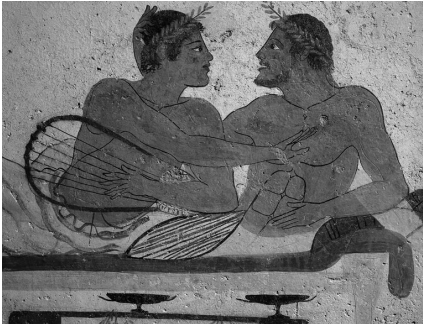
\includegraphics[scale = 0.4]{../images/TheLovers.PNG}
    \caption{The Lovers; detail of a fresco from the Tomb of the Diver (c. 480-470 BCE)}
    \label{fig:love}
\end{figure}

This has appeared in many scholarly works of homosexuality in the ancient world. However, based on our understanding of the ancient Greek past, this depiction is neither a representation of homosexuality nor of gayness unless we are to speak in an anachronistic (belonging to a period other than that portrayed), essentialist (objects have an underlying reality or true nature that one cannot observe directly) view.

\begin{qst}
    Should we then use the broader, more flexible category of queer, which denotes a site of marginalization from and resistance to dominant culture, to try to link the male-male eroticism of the past to the homosexuality of the present?
\end{qst}

If the paintings were modern they would fit into the context of ``queer." Indeed, the ultimate setting for the \textbf{er$\overline{\text{o}}$menos} and \textbf{erast$\overline{\text{e}}$s} in the painting is a homoerotic, homosocial afterlife.

\begin{rmk}
    In the context of their time, the paintings invite us to a space that was a privileged location of the Greek patriarchy---the symposium.
\end{rmk}

Indeed, the Tomb of the Diver paintings are like the pederastic (depicting intimacy between a male and young boy, usually in his teens) symposium scenes found on Attic pottery (pottery from the \textbf{Attica}, a historical region encompassing Athens) and described in philosophical and other Greek treatises. 

\begin{nte}
    The author argues that Ancient Greek societies were \textbf{homonormative} in that they privileged males and prioritized relationships between men through the institution of pederasty.
\end{nte}

The paintings show local Italic influences, especially of death sexuality, and banqueting that seem to have been borrowed from the Etruscans (civilization which controlled a majority of the Italian peninsula). However, in Etruscan depictions the male-female couple is privileged, but in the Tomb of the Diver it is the male-male couple that stands out. This suggests the Greeks of Poseidonia borrowed heavily from Etruscan conceptions of the afterlife, but adapted these ideas to suit their own solial milieu.

\begin{rmk}
    The eroticism and eschatology of the iconography of the Tomb of the Diver suggests the deceased was an initiate of the \textbf{Orphic cult}.
\end{rmk}

The Orphic cult followed a collection of beliefs and practices related to the mythical poet \textbf{Orpheus}. Previous scholarship ignored or subordinated the eroticism of the paintings to other concerns. The main exception to this is the analysis of \textbf{Cerchiai (1987)}, who instead subordinates the eschatological themes to the erotic. The author attempts to provide a more balanced approach.

\begin{nte}
    The author argues that the Orphic rites were, in much more of a Greek than an Etruscan fashion, both homosocial and homoerotic. In Orphic though, the symposium served both as a means to worship Dionysus and other gods in this life, and as an image of the eternal hereafter in the next life.
\end{nte}




\subsection{The Paintings}


The paintings in the Tomb have been dated to approximately \textbf{480-470 BCE} based on pottery in the tomb. The two long sided slabs depict partygoers lounging on couches at what has been identified as a symposium.

\begin{figure}[H]
    \centering
    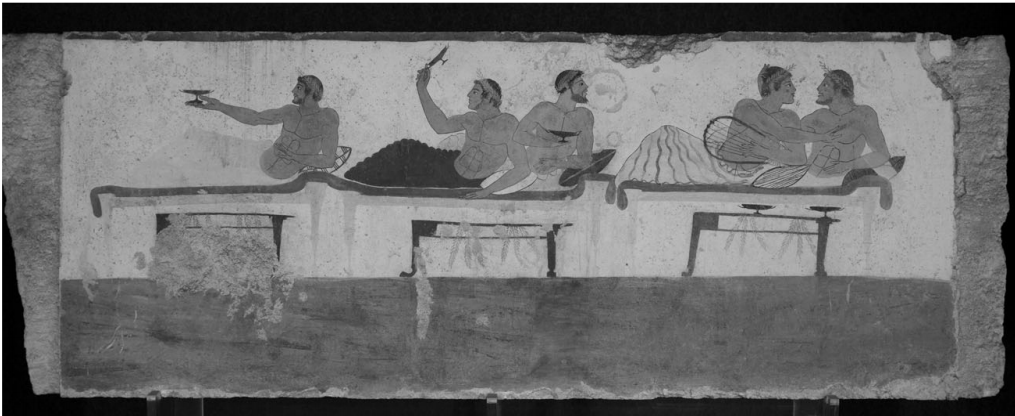
\includegraphics[scale = 0.3]{../images/North.PNG}
    \caption{North wall of Tomb of the Diver}
    \label{fig:north}
\end{figure}

\begin{figure}[H]
    \centering
    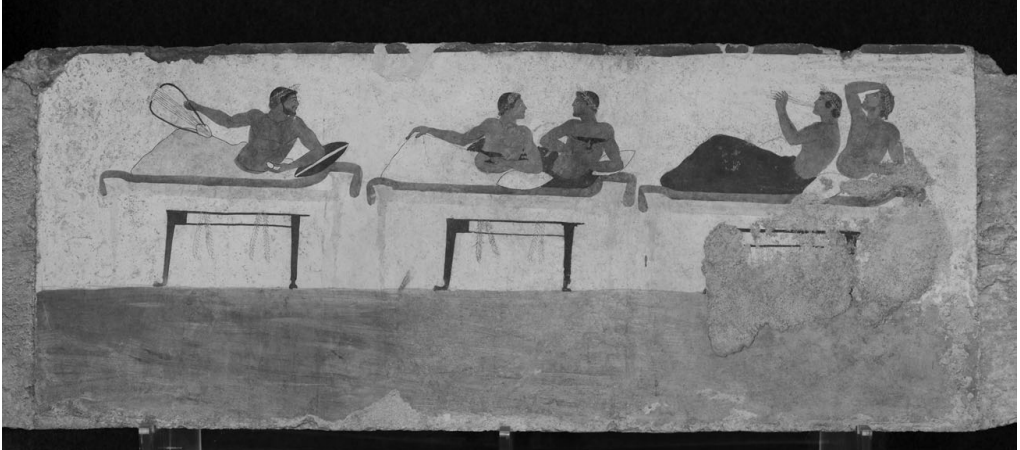
\includegraphics[scale = 0.3]{../images/South.PNG}
    \caption{South wall of Tomb of the Diver}
    \label{fig:south}
\end{figure}

Most of the male guests appear in couples, and the celebrated pair in Figure \ref{fig:love} have been labeled \textbf{gli amanti ``the lovers"} by Mario Napoli, the archeologist who discovered the tomb. On the opposite wall one of the symposiasts is playing music while his couchmate holds his hand to his forehead, a gesture which has been interpreted to indicate a state of ecstasy. The symposiast on the left in Figure \ref{fig:south} is holding an egg, which has been identified as a symbol of the Greek Orphic religious movement (it symbolizes the belief in eventual reunification with a divine source---Phanes, also called Eros, the creator of all things, was an androgynous being who was originally thought to have hatched from a shell). On the middle couch (\textbf{klin$\overline{\text{e}}$}) of Figure \ref{fig:north} the symposiast has raised his \textbf{kylix} (wine drinking cup) at an angle indicating that he is playing \textbf{kottabos} (similar to modern-day darts). The dregs offered in kottabos in a symposium were done so in the name of an \textbf{er$\overline{\text{o}}$menos}.

\begin{figure}[H]
    \centering
    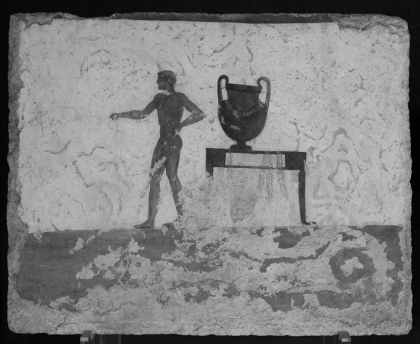
\includegraphics[scale = 0.3]{../images/East.PNG}
    \caption{East wall of Tomb of the Diver. Depicts a youth walking from a garlanded krater which appears to contain wine. The youth is most likely the designated wine pourer for the guests.}
    \label{fig:east}
\end{figure}


\begin{figure}[H]
    \centering
    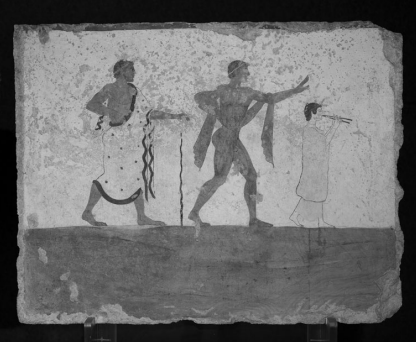
\includegraphics[scale = 0.3]{../images/West.PNG}
    \caption{West wall of Tomb of the Diver. A procession of symposiasts led by a female flautist followed by a naked youth with a blue scarf draped over his arms and a clothed bearded man.}
    \label{fig:west}
\end{figure}



\begin{figure}[H]
    \centering
    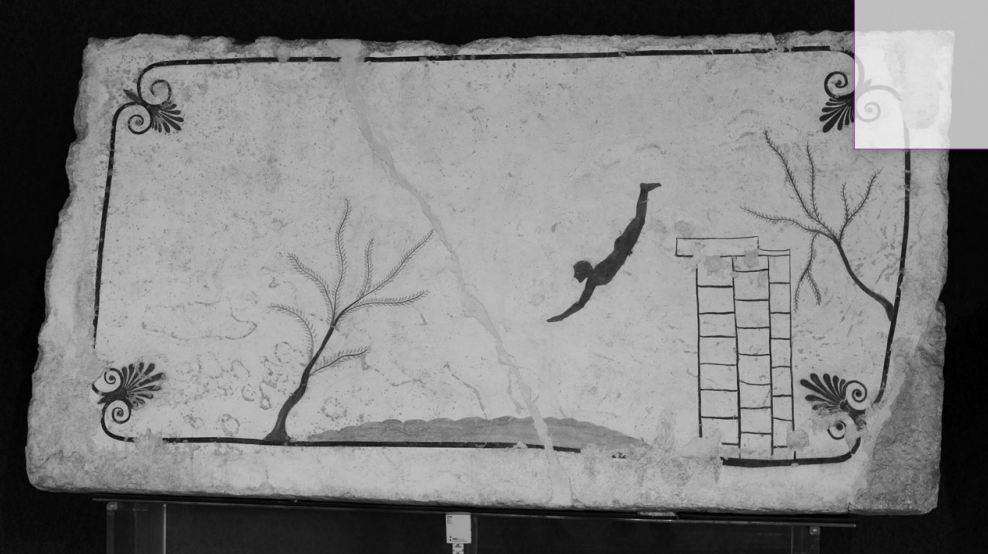
\includegraphics[scale = 0.3]{../images/Cover.PNG}
    \caption{Slab cover of Tomb of the Diver. A naked young man is pictured diving into a body of water.}
    \label{fig:slab}
\end{figure}


The Poseidonian paintings in the Tomb of the Diver, despite similarities in the symposium scenes, otherwise fall outside the norms of \textbf{Attic art}. The association of the symposium with the afterlife and of eschatology with eroticism are reflective of Etruscan influence, as \textbf{Pontrandolfo (1996)} has argued:

\begin{quotation}
    While full of Greek conceptual models, the paintings in the Diver's Tomb are in fact an exception, even as far as their contents are concerned, because they do not mirror the typical mental attitude of Greeks who would normally never decorate the interior of tombs with paintings, nor place the world of death together with that of the symposium, for the two worlds contradict each other. The homosociality of the symposium participants, nevertheless, is very Greek.
\end{quotation}

As with other Attic symposium scenes, the only female in the frescoes is a young flute girl. In contrast, Etruscan paintings show women, probably wives, at symposia.

\begin{figure}[H]
    \centering
    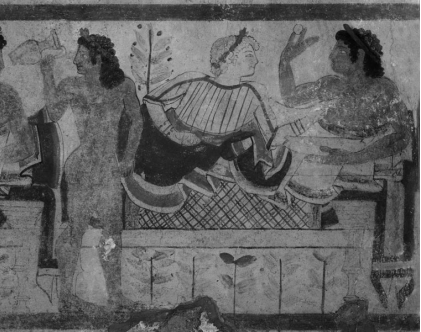
\includegraphics[scale = 0.3]{../images/Leopards.PNG}
    \caption{Tomb of the Leopards}
    \label{fig:leo}
\end{figure}

\begin{rmk}
    No other comparable funerary paintings from the fifth century have been discovered in the vicinity of Poseidonia.
\end{rmk}

Other painted tombs from the fourth century BCE have been found, but they date to the period after the Lucanian invasion/conquest of Poseidonia (when the name of the city was changed to Paestum), thus after the period of Greek rule of the \textbf{polis} of Poseidonia. Nonetheless, fourth-century male burials are usually accompanied by \textbf{kraters} and other wine vessels which suggest that, for men, the afterlife might include a symposium.

\subsection{Eschatology of the tomb's iconography}

Note that \textbf{eschatology} is the part of theology concerned with death, judgement, and the final destiny of the soul and humankind. 

\textbf{Napoli} interpreted the dive scene as \textbf{Pythagorean}, representing the purifying passage of the soul through water. But this fails to account for the relationship of the diver to the symposium scene. 

\textbf{Bianchi-Bandinelli (1970)} has asserted that the symposium scenes represent the heroic afterlife in the Isles of the Blessed beyond the western limits of the Mediterranean described by \textbf{Hesiod}, that the structure from which the diver leaps representes the \textbf{Pillar of Heracles}, and that the body of water he plunges into is the Atlantic Ocean, which represented the limits of the known world to the Greeks. However several centuries separate the time of Hesiod and the tomb, and the body of water into which the diver plunges looks much more like a small lake or spring than an ocean.

Note the diver, the association of the symposium with the afterlife, and the procession of the deceased are all themes that surface in Etruscan funerary art. The Greek colony of Poseidonia lay just to the south of Naples, and the polis shared a border along the River Sele, with ancient Campania. Campania was already ``deeply Etruscanized" by the end of the seventh century BCE, when Poseidonia was founded. The inhabitants of Poseidonia mingled and possibly intermarried with Etruscans and other native inhabitants of the region, so the influx of Etruscan eschatology into the region is not surprising. Inscriptions on an \textbf{olp$\overline{\text{e}}$} manufactured at Poseidonia and found at Fratte di Salerno contains short erotic verses involving persons with Greek, Etruscan, and other Italic names.

Although the association of the symposium with the afterlife is at first an Italic/Etruscan feature, the paintings do represent the attitude of at least some Greeks---those Greeks called ``Orphics" who followed the teachings of \textbf{Musaeus}. Indeed, Plato described the Orphic conception of the afterlife as a banquet where the reward is eternal drunkenness (attributed to Musaeus, who was either a son or friend to Orpheus).

\begin{nte}
    Orpheus was a prophet of Dionysus, and hence the ``Orphic" cult was associated with and perhaps even synonymous with the Dionysiac/Bacchic mysteries in ancient Southern Italy.
\end{nte}

Orphic beliefs demonstrate a number of commonalities with Etruscan eschatology, including:

\begin{enumerate}
    \item[(1)] a procession of the dead to a blessed afterlife;
    \item[(2)] a need to either pass through or drink water to reach that afterlife;
    \item[(3)] the representation of that afterlife as a banquet or symposium.
\end{enumerate}

By the fourth century BCE Plato refers to the ``Orphic" idea of the afterlie as a symposium being a reward for the just, whereas the unjust went to the house of Hades as punishment for their wrongdoings. This suggests that the Etruscan idea of the afterlife was borrowed by Greeks who adapted it for their own needs in the Orphic cult.

\begin{rmk}
    This is a radical departure from archaic Greek religion where humans went to the gloomy ``land of the shadows" described by Homer, save for a select few of the heroic race you transcended mortality to dwell in the paradise of the Elysian fields at the end of the earth described by Hesiod. On the other hand in Orphic belief the afterlife was a reunion with the gods, in the form of a symposium.
\end{rmk}

Some other Orphic initiates in nearby Greek colonies were buried with a tablet, considered by archeologists to be a type of passport which would give the Orphic initiate access to the afterlife. A fifth-century tablet found in Hipponium in Souther Italy contained a small text:

\begin{quotation}
    This (dictate) is sacred to Memory (for the \textbf{mystes} [initiate]) on the point of death. You will go to the well-built house of Hades, where, on the right, there lies a spring, and next to that a white cypress tree stands. There the souls of the dead seek refreshment. Do not even approach this spring. Beyond it you will find the cold water that runs from the lake of Memory, with its keeper to the fore, and they will ask you, with clear penetration, what you seek in the shades of murky Hades. Reply: ``I am the son of the Earth and of starry Heaven; I burn with thirst and I am fainting; quick, give me to drink the cold water that comes from the lake of Memory. They are merciful, as the king of the underworld wills, and will give you to drink from the lake of Memory; and when you have drunk you will travel the sacred path where the other \textbf{mystai} and \textbf{bakkhoi} proceed in glory."
\end{quotation}

In this context the procession depicted on the west wall of the tomb may be none other than a sacred procession of \textbf{bakkhoi} as mentioned in the tablet above.

However, some skepticism over the ``Orphic" associations in this text have been expressed because the deceased buried with it was a woman. What we can loosely term ``Orphic/Dionysiac" cults were marked by sex-segregated rites.

The elements of water and earth are also invoked in what \textbf{Clement of Alexandria} alleges is the writing of Orpheus himself:

\begin{quotation}
    Water is death for souls, But from water comes earth, from earth again water, and thence soul, rushing to all the ether.
\end{quotation}

Both Orpheus and Dionysus journey to the underworld and return from it in Greek myth, and it stands to reason that both of these mythical characters, the god and his prophet, were believed to have the power to intercede on behalf of the dead with the rulers of the underworld.

\subsection{The symposium and Orphic rites: Higher forms of knowledge, homosociality, and homoeroticism}

Orphic/Dionysiac mystery rites ultimately sought to provide the initatie with a better afterlife through the purification provided by traveling Orphic priests, or \textbf{orpheotelestai}. From a tablet in the Black Sea colony of Olbia dating to the fifth century BCE, one finds the text ``life death life truth," which seems to argue for reincanation at least once before reaching the Orphic afterlife of ``truth." ``Liberation from the wheel of life" in Orphism could be achieved, it was thought, through religious rites.

Beginning in the 480s BCE, and hence relevant to the Tomb of the Diver paintings, Attic vases show Orpheus surrounded by males only. \textbf{Phanocles} explains that Orpheus introduced ``male love" (\textbf{er$\overline{\text{o}}$tas arrenas}) to the Thracians. Eventually the Thracian women killed Orpheus out of jealousy for taking their husbands away from them. In terms of the pederasty and homosociality, the ``Orphic rite" has much in common with the Greek concept of the symposium.

According to \textbf{Cerchiai} the reveler would obtain access to higher forms of knowledge through the symposium. In the symposium, ``the phrase `wine and truth' was proverbial for those who talked frankly while inebriated."

\begin{nte}
    Sympotic discussions strove both to enlighten one's contemporaries with regard to politics but even more to educate the \textbf{er$\overline{\text{o}}$menoi} present, just as the Orphic rite strove to educate the initiate as to how to find an eternity of sympotic pleasure.
\end{nte}

The sexuality displayed is consistent with a neschatological Orphic reading. \textbf{Cerchiai} suggests that the procession on the west wall of the tomb is an erotic hunt, in which the older bearded man is chasing the younger, nude man.


\subsection{Ancient Paintings, Modern Queerness}

The sympotic scenes denote what is, for all intents and purposes, a specifically ancient context. The symposium scene was more than a drinking party; it was a ritual, wherein a libation was poured to the god Dionysus, paeans were sung, and divination was sought through the game of kottabos. The Tomb of the Diver symposium seems to represent both the best of this life and hereafter, given Plato's description of the Orphic afterlife as sympotic. 

\begin{rmk}
    In the social development of a Greek citizen, the youth was meant to begin his sexual and social development as an \textbf{er$\overline{\text{o}}$menos}, then, when his beard came in, to become the \textbf{erast$\overline{\text{e}}$s}, and finally, around the age of $30$, to give up youthful same-sex \textbf{er$\overline{\text{o}}$s} and marry.
\end{rmk}

This was normative. Understanding ``queerness" as being identified with marginalization and transgression, the author argues that there is nothing ``queer" going on, but instead the paintings should be called ``homonormative," in the ancient Greek context, defining the centrality of social and/or erotic relationships among men to the institutions such as the symposium, that reify and promote exclusive male privilege in the power structures of society.

According to \textbf{Cohen (1991)}:
\begin{quotation}
    when an Athenian man courts a boy he does so according to the normative expectations ofthe boy, his family, and the community of which he is a part (all social interaction is normatively structured by such expectations, though these expectations may conflict or reflect moral ambivalences about the conduct). Yet the norms reflected in such expectations do not simply determine his behavior. He possesses the knowledgeability that almost all individuals have about the norms, values, beliefs, and practical expectations of the society in which they live. This knowledgeability enables individuals to influence evaluations of their behavior by interpreting and manipulating their words and deeds and the normative categories by which they are judged.
\end{quotation}

While little is known of the customs and social history of ancient Poseidonia, its mother city of \textbf{Sybaris}, itself an \textbf{Achaean colony} that was known for its wealth and luxurious way of life in antiquity had a few more details. The inhabitants of Sybaris were the most indulgent of the Western Greeks. The Sybarites were known to like and have befriended the Etruscans to the north and the Ionians to the east. 

\begin{qst}
    Could this indicate Etruscan influence on Poseidonian sexuality? 
\end{qst}

Note the Poseidonians lived between the Sybarites and the Etruscans, and had absorbed some of the Etruscan ideology of the afterlife into their own eschatology. Inscriptions on an \textbf{olp$\overline{\text{e}}$} made in Poseidonia nad found in a tomb at nearby Fratte di Salerno suggests that same-sex activity was enjoyed between Greeks and Etruscans:

\begin{quotation}
    Apollodorus loves Kscylla 

    Wolchas buggers Apollodorus

    Onatas loves Nikso

    Hybrichus has love Parmynio.
\end{quotation}

Five males (Apollodorus, Wolchas, Onatas, Hubrichus, and Parmynio) and two females (Ksylla and Nikso) are named. Athenaeus points out that the Etruscan men enjoyed sex with both boys (\textbf{paides}) and young men (\textbf{meirakia}), a term that refers approximately to twenty-yera-old males.

\subsection{Conclusion}

The paintings analyzed suggest that the idea of a drunken, sexy hereafter derived from an Etruscan context was imported into Greek thought and altered to fit Greek norms of homosociality and pederasty in the ``Orphic" religious movement. The Tomb of the Diver paintings display a relationship between male-male eroticism and the afterlife that is Orphic.

The Tomb of the Diver paintings show a pederastic ideal, even if it is not as stringent as the Athenian model. The close proximity of Poseidonia to Etruscan and othe Italic communities may offer a rationale for this phenomenon.





\section{Notes on Analysis and Societal Context}
\label{sec:SocCont3}

\begin{rmk}
    The author begins by describing the five paintings before preceeding to a survey of the secondary scholarship on the paintings, and then presenting their own interpretations. Finally, they return to the question of the use of images to mark homosexuality or gay identity, and argue that the scene in the painting is neither gay nor queer, but rather offers a ``homonormative" paradigm.
\end{rmk}

\begin{nte}
    As the author notes, to be useful for analysis of ancient Greek evidence queer theory must be adapted and refined as concepts like ``heteronormative" do not really apply.
\end{nte}



%
% \begin{acknowledgement}
% If you want to include acknowledgments of assistance and the like at the end of an individual chapter please use the \verb|acknowledgement| environment -- it will automatically render Springer's preferred layout.
% \end{acknowledgement}
%
% \section*{Appendix}
% \addcontentsline{toc}{section}{Appendix}
%


% Problems or Exercises should be sorted chapterwise
\section*{Problems}
\addcontentsline{toc}{section}{Problems}
%
% Use the following environment.
% Don't forget to label each problem;
% the label is needed for the solutions' environment
\begin{prob}
\label{prob1}
A given problem or Excercise is described here. The
problem is described here. The problem is described here.
\end{prob}

% \begin{prob}
% \label{prob2}
% \textbf{Problem Heading}\\
% (a) The first part of the problem is described here.\\
% (b) The second part of the problem is described here.
% \end{prob}

%%%%%%%%%%%%%%%%%%%%%%%% referenc.tex %%%%%%%%%%%%%%%%%%%%%%%%%%%%%%
% sample references
% %
% Use this file as a template for your own input.
%
%%%%%%%%%%%%%%%%%%%%%%%% Springer-Verlag %%%%%%%%%%%%%%%%%%%%%%%%%%
%
% BibTeX users please use
% \bibliographystyle{}
% \bibliography{}
%


% \begin{thebibliography}{99.}%
% and use \bibitem to create references.
%
% Use the following syntax and markup for your references if 
% the subject of your book is from the field 
% "Mathematics, Physics, Statistics, Computer Science"
%
% Contribution 
% \bibitem{science-contrib} Broy, M.: Software engineering --- from auxiliary to key technologies. In: Broy, M., Dener, E. (eds.) Software Pioneers, pp. 10-13. Springer, Heidelberg (2002)
% %
% Online Document

% \end{thebibliography}

